\documentclass[12pt,a4paper]{article}
\usepackage[utf8]{inputenc}
\usepackage[T1]{fontenc}
\usepackage[english]{babel}
\usepackage[left=2cm,right=2cm,top=2cm,bottom=2cm]{geometry}
\usepackage{lmodern}
\usepackage{parskip}

% Mathematical packages
\usepackage{amsmath, amssymb, amsthm, mathtools, physics}
\usepackage{siunitx}

% Graphics and diagram packages
\usepackage{graphicx}
\usepackage{tikz, tikz-feynman}
\usepackage{pgfplots}
\pgfplotsset{compat=1.18}

% Tables and formatting
\usepackage{booktabs}
\usepackage{array}
\usepackage[table,xcdraw]{xcolor}

% Theorems and references
\usepackage{thmtools}

% Boxes and special formatting
\usepackage{tcolorbox}
\tcbuselibrary{theorems, breakable}

% Hyperlinks and PDF metadata
\usepackage{hyperref}

\usepackage{cleveref}
\hypersetup{
	colorlinks=true,
	linkcolor=blue,
	citecolor=blue,
	urlcolor=blue,
	pdftitle={Time-Mass Duality Theory (T0 Model)},
	pdfauthor={Johann Pascher},
	pdfsubject={Theoretical Physics},
	pdfkeywords={T0 Model, natural units, time-mass duality}
}

% Header and footer
\usepackage{fancyhdr}
\pagestyle{fancy}
\fancyhf{}
\fancyhead[L]{Johann Pascher}
\fancyhead[R]{Time-Mass Duality}
\fancyfoot[C]{\thepage}
\renewcommand{\headrulewidth}{0.4pt}
\renewcommand{\footrulewidth}{0.4pt}

% Table of contents styling
\usepackage{tocloft}
\renewcommand{\cftsecfont}{\color{blue}}
\renewcommand{\cftsubsecfont}{\color{blue}}
\renewcommand{\cftsecpagefont}{\color{blue}}
\renewcommand{\cftsubsecpagefont}{\color{blue}}
\setlength{\cftsecindent}{1cm}
\setlength{\cftsubsecindent}{2cm}

% Custom commands (consistent)
\newcommand{\Tfield}{T(x)}
\newcommand{\DcovT}[1]{\Tfield D_\mu #1 + #1 \partial_\mu \Tfield}
\newcommand{\DhiggsT}{\Tfield (\partial_\mu + ig A_\mu) \Phi + \Phi \partial_\mu \Tfield} % Uniform definition
\newcommand{\HiggsLagr}{\mathcal{L}_{\text{Higgs-T}}}
\newcommand{\FermionLagr}{\mathcal{L}_{\text{Fermion-T}}}
\newcommand{\BosonLagr}{\mathcal{L}_{\text{Boson-T}}}
\newcommand{\Mpl}{M_{\text{Pl}}}
\newcommand{\alphaEM}{\alpha_{\text{EM}}}
\newcommand{\betaT}{\beta_{\text{T}}}
\newcommand{\alphaW}{\alpha_{\text{W}}}
\newcommand{\Tzerot}{T_0(\Tfield)}
\newcommand{\Tzero}{T_0}
\newcommand{\vecx}{\vec{x}}
\newcommand{\gammaf}{\gamma_{\text{Lorentz}}}

% Theorem environment definition
\newtheorem{theorem}{Theorem}[section]
\newtheorem{lemma}{Lemma}[section]

\begin{document}
	
	\title{Time-Mass Duality Theory (T0 Model): \\ Derivation of Parameters \(\kappa\), \(\alpha\) and \(\beta\)}
	\author{Johann Pascher}
	\date{April 10, 2025}
	
	\maketitle
	
	\section*{Introduction}
	
	This paper examines the connection between natural unit systems and dimensionless constants in the T0 model of time-mass duality theory. It is argued that the parameter \(\beta \approx 0.008\) in the temperature-redshift relation \(T(z) = T_0 (1+z)(1+\beta\ln(1+z))\) can be set to \(\beta = 1\) in natural units, analogous to Wien's constant \(\alpha_W\) \cite{pascher_temp_2025}. Additionally, the parameters \(\kappa\), \(\alpha\) and \(\beta\) of the T0 model are derived in detail and linked to cosmological implications. For a further analysis of the consistency when simultaneously setting the fine structure constant \(\alphaEM = 1\) and the parameter \(\betaT = 1\), see \cite{pascher_alphabeta_2025}.
	
	\tableofcontents
	\newpage
	
	\section{Dimensionless Parameters in Fundamental Theories}
	
	\subsection{Historical Development and Principles}
	
	Physics shows an evolution towards unit systems in which natural constants are set to 1:
	\begin{itemize}
		\item Maxwell: \(c\) as a fundamental constant
		\item Theory of Relativity: \(c = 1\)
		\item Quantum Mechanics: \(\hbar = 1\)
		\item Quantum Gravitation: \(G = 1\)
	\end{itemize}
	Dimensionless parameters should be simple (e.g., 1, \(\pi\)). \(\betaT^{\text{SI}} \approx 0.008\) suggests a non-optimal system.
	
	\subsection{The Significance of the "Right" Natural Units}
	
	Complex values like \(\betaT^{\text{SI}} \approx 0.008\) suggest that the formulation is not fundamental. Historical examples:
	\begin{itemize}
		\item \(c = 1\) in appropriate units
		\item \(\hbar = 1\) in quantum units
		\item \(G = 1\) in Planck units
	\end{itemize}
	
	\section{The Characteristic Length Scale \(r_0\)}
	
	\subsection{Redefinition of \(r_0\) in Natural Units}
	
	The length scale \(r_0\) is defined as \(r_0 = \xi \cdot l_P\), where \(\xi\) is a dimensionless constant and \(l_P = \sqrt{\frac{\hbar G}{c^3}}\) is the Planck length. In natural units (\(\hbar = c = G = 1\)), \(l_P = 1\), thus \(r_0 = \xi\).
	
	From \(\betaT^{\text{nat}} = 1\) and:
	
	
	\begin{equation}
		\betaT^{\text{nat}} = \frac{\lambda_h^2 v^2}{4\pi^2 \lambda_0^2 \alpha_0}
	\end{equation}
	follows:
	\begin{equation}
		\xi = \frac{\lambda_h^2 v^2}{16\pi^3 m_h^2} \approx 1.33 \times 10^{-4}
	\end{equation}
	\begin{equation}
		r_0 \approx \frac{1}{7519} \cdot l_P
	\end{equation}
	
	\subsection{Physical Interpretation}
	
	\(r_0\) is the interaction length between \(\Tfield\) and the Higgs field:
	\begin{itemize}
		\item Correlation of fluctuations
		\item Transition between quantum and classical gravitation
		\item Coupling to the electroweak sector
	\end{itemize}
	This indicates a Planck-scale connection.
	
	\subsection{Conversion Between Natural Units and SI Units}
	
	\begin{align}
		r_{0,\text{SI}} &= \xi \cdot l_{P,\text{SI}} \\
		&= 1.33 \times 10^{-4} \cdot \SI{1.616255e-35}{\meter} \\
		&\approx \SI{2.15e-39}{\meter}
	\end{align}
	\begin{align}
		\betaT^{\text{SI}} &= \betaT^{\text{nat}} \cdot \frac{r_{0,\text{nat}}}{r_{0,\text{SI}}/l_{P,\text{SI}}} \\
		&= 1 \cdot \frac{\xi \cdot l_{P,\text{SI}}}{r_{0,\text{SI}}} \\
		&\approx 0.008
	\end{align}
	
	\subsection{Consistency with the Cosmological Length Scale \(L_T\)}
	
	\begin{equation}
		L_T \sim \frac{\Mpl}{m_h^2 v} \approx \SI{6.3e27}{\meter}
	\end{equation}
	\begin{equation}
		\frac{r_0}{L_T} \sim \frac{\lambda_h^2 v^4}{16\pi^3 \Mpl} \approx 3.41 \times 10^{-67}
	\end{equation}
	
	This ratio is remarkable as it is of the order of \((m_e/M_{Pl})^2\), possibly indicating a deeper connection to the electron mass.
	
	\section{Parameter Derivations in the T0 Model}
	
	\subsection{Derivation of \(\kappa\)}
	
	\begin{theorem}[Derivation of \(\kappa\)]
		In natural units:
		\begin{equation}
			\kappa^{\text{nat}} = \betaT^{\text{nat}} \frac{y v}{r_g^2}, \quad r_g = \sqrt{\frac{M}{a_0}}
		\end{equation}
		
		where \(r_g\) is the gravitational radius defined by the mass \(M\) and the MOND acceleration scale \(a_0 \approx \SI{1.2e-10}{\meter\per\second\squared}\).
		
		The dimensional analysis yields:
		\begin{align}
			[\kappa^{\text{nat}}] &= [1] \cdot \frac{[1] \cdot [E]}{[L]^2} \\
			&= \frac{[E]}{[E^{-2}]} \\
			&= [E]
		\end{align}
		
		In SI units:
		\begin{equation}
			\kappa_{\text{SI}} = \betaT^{\text{SI}} \frac{y v c^2}{r_g^2} \approx \SI{4.8e-11}{\meter\per\second\squared}
		\end{equation}
	\end{theorem}
	
	\subsection{Derivation of \(\alpha\)}
	
	\begin{theorem}[Derivation of \(\alpha\)]
		In natural units:
		\begin{equation}
			\alpha^{\text{nat}} = \frac{\lambda_h^2 v}{L_T^2}
		\end{equation}
		
		The dimensional analysis yields:
		\begin{align}
			[\alpha^{\text{nat}}] &= \frac{[1] \cdot [E]}{[E^{-2}]} \\
			&= [E]
		\end{align}
		
		In SI units:
		\begin{equation}
			\alpha_{\text{SI}} = \frac{\lambda_h^2 v c^2}{L_T^2} \approx \SI{2.3e-18}{\per\meter}
		\end{equation}
		where \(\lambda_h\) is the Higgs self-coupling.
	\end{theorem}
	
	\subsection{Derivation of \(\beta\): Fundamental Electromagnetic Derivation}
	
	\begin{theorem}[Electromagnetic Derivation of \(\beta\)]
		The fundamental derivation of the parameter \(\beta_T\) is based on the electromagnetic vacuum constants \(\mu_0\) and \(\varepsilon_0\):
		
		In electromagnetic theories, the relationship holds:
		\begin{equation}
			c^2 = \frac{1}{\mu_0 \varepsilon_0}
		\end{equation}
		
		The parameter \(\beta_T\) can be defined with dimensional consistency as:
		
		\begin{equation}
			\beta_T^{\text{nat}} = \frac{\lambda_h^2 v^2}{16\pi^3 m_h^2 \xi} = \frac{\hbar}{m_h c}\)
			\item \(\alpha_0\): dimensionless coupling constant of the T0 model $[1]$
			\item \(k\): dimensionless exponent that yields \(\beta_T^{\text{nat}} = \frac{\lambda_h^2 v^2}{16\pi^3 m_h^2 \xi} =0\)
		\end{itemize}
		
		The dimensional analysis yields:
		\begin{align}
			[\beta_T^{\text{nat}}] &= [\lambda_h^2] \cdot [v^2] \cdot [\lambda_0^{-2}] \cdot [\alpha_0^{-1}] \cdot [(\mu_0/\varepsilon_0)^{k}] \\
			&= [1] \cdot [E^2] \cdot [E^{-2}] \cdot [1]^{-1} \cdot [1] \\
			&= [1]
		\end{align}
		
		This derivation shows that \(\beta_T\) is a dimensionless parameter, consistent with its role as a fundamental coupling constant in the T0 model.
	\end{theorem}
	
	In natural units with \(\hbar = c = 1\) and \(\mu_0 = \varepsilon_0 = 1\), we get \(\beta_T^{\text{nat}} = \frac{\lambda_h^2 v^2}{16\pi^3 m_h^2 \xi} = 1\) in the theory of relativity. The corresponding SI-units form is derived through conversion:
	\begin{equation}
		\beta_T^{\text{SI}} \approx 0.008
	\end{equation}
	
	The discrepancy between the values is an artifact of the unit system and not a physical inconsistency.
	
	\subsection{From Natural to SI Units}
	
	\begin{theorem}[Alternative Derivation of \(\beta\)]
		In natural units: \(\betaT^{\text{nat}} = 1\). Perturbatively:
		\begin{equation}
			\betaT^{\text{nat}} = \frac{\lambda_h^2 v^2}{4\pi^2 \lambda_0^2 \alpha_0}
		\end{equation}
		In SI units:
		
		\begin{equation}
			\betaT^{\text{SI}} = \betaT^{\text{nat}} \cdot \frac{\lambda_h^2 v^2}{4\pi^2 \lambda_0^2 \alpha_0} \approx 0.008
		\end{equation}	
		
		where \(\lambda_0\) is a characteristic wavelength and \(\alpha_0\) a coupling constant of the T0 model.
	\end{theorem}
	
	Here, \(\lambda_0\) and \(\alpha_0\) are parameters related to the structural constant of the T0 model. It should be noted that \(\alpha_0\) is not necessarily identical to the fine structure constant \(\alphaEM\), although a relationship between the two might exist (see \cite{pascher_alphabeta_2025}).
	
	\subsection{Application: Wavelength-Dependent Redshift and Temperature Evolution}
	
	From setting \(\betaT^{\text{nat}} = 1\), the redshift-wavelength relation follows:
	
	\begin{equation}
		z(\lambda) = z_0 \left(1 + \betaT^{\text{SI}} \ln \frac{\lambda}{\lambda_{\text{ref}}}\right)
	\end{equation}
	And the temperature-redshift relation:
	\begin{equation}
		T(z) = T_0 (1 + z) (1 + \betaT^{\text{SI}} \ln(1 + z))
	\end{equation}
	
	\subsubsection{Feynman Diagram Analysis}
	
	\begin{center}
		\feynmandiagram [horizontal=a to b] {
			a [particle=\(\gamma\)] -- [photon] b -- [photon] f [particle=\(\gamma\)],
			b -- [scalar, half left] c -- [scalar, half left] b,
			c -- [photon] d,
		};
	\end{center}
	
	\section{Quantum Theoretical Determination of the Parameter \(\betaT\)}
	
	The quantum field theoretical analysis of the T0 model yields a perturbative value for the dimensionless parameter \(\betaT^{\text{SI}} \approx 0.008\) in SI units, which is consistent with cosmological observations. This value was derived through a perturbative treatment of the interaction between the intrinsic time field \(\Tfield\) and matter, with the fundamental time-mass duality \(m = \frac{\hbar}{\Tfield c^2}\) as a starting point. In particular, it is shown that \(\betaT^{\text{SI}}\) reflects the strength of the coupling between time field fluctuations and cosmic expansion, manifesting in a wavelength-dependent redshift \(z(\lambda) = z_0 \left(1 + \betaT \ln \frac{\lambda}{\lambda_0}\right)\) as well as in modified rotation curves of galaxies. A comprehensive presentation of this derivation, including experimental verifiability through cosmological measurements, can be found in \cite{pascher_emergente_gravitation_2025}, especially in the section "Experimental Tests and Predictions."
	
	A deeper theoretical consideration reveals, however, that in natural units (\(\hbar = c = 1\)), the parameter \(\betaT^{\text{nat}} = 1\) is equivalent. This equivalence arises from the scaling property of the time-mass duality, which enables a unified representation of physical quantities in natural units. In the T0 model, mass is defined as an inverse function of the time field, and the choice of natural units eliminates dimensionful constants such as \(\hbar\) and \(c\), giving \(\betaT\) a universal meaning. In \cite{pascher_emergente_gravitation_2025}, section "Natural Units in the T0 Model," it is shown that this transition is not merely a mathematical simplification, but also reveals fundamental connections between time, mass, and gravitation. For example, the field equation 
	\begin{equation}
		\nabla^2 \Tfield = -\kappa \rho(\vecx) \Tfield^2
	\end{equation}
	in natural units leads to a direct connection between the mass density \(\rho(\vecx)\) and the gradients of the time field that generate emergent gravitation.
	
	The discrepancy between \(\betaT^{\text{SI}} \approx 0.008\) and \(\betaT^{\text{nat}} = 1\) is thus not a contradiction, but an artifact of the chosen unit systems. In SI units, \(\betaT\) is scaled by the specific values of \(\hbar\), \(c\), and other constants, while natural units eliminate this scaling and present \(\betaT\) as a unified coupling constant. This duality of representation has far-reaching implications: While \(\betaT^{\text{SI}}\) is directly linked to observable quantities such as cosmic acceleration and galaxy dynamics, \(\betaT^{\text{nat}}\) provides a theoretical foundation for the unification of the T0 model with other physical theories, such as the Higgs mechanism or entropic gravitation, as further elaborated in \cite{pascher_emergente_gravitation_2025}. Future work could aim to refine the quantum theoretical derivation of \(\betaT\) through non-perturbative methods to further substantiate the consistency between these two values.
	
	\section{Interpretation and Coherence of Natural Parameters}
	
	\subsection{Hierarchy of Units and Dimensionless Constants}
	
	\begin{enumerate}
		\item Natural constants: \(c = \hbar = G = k_B = 1\)
		\item Dimensionless parameters: \(\alphaEM \approx 1/137\), \(\alpha_W \approx 2.82\) \cite{pascher_temp_2025}, \(\betaT^{\text{nat}} = 1\)
		\item Length scales: \(r_0 = \xi \cdot l_P\), \(\xi \approx 1.33 \times 10^{-4}\); \(L_T = \zeta \cdot l_P\), \(\zeta \sim 10^{62}\)
	\end{enumerate}
	
	\subsection{Ratios Between Length Scales in the T0 Model}
	
	\begin{itemize}
		\item \(l_{P,\text{SI}} \approx \SI{1.616e-35}{\meter}\)
		\item \(\lambda_h \approx \SI{1.576e-18}{\meter}\)
		\item \(r_{0,\text{SI}} \approx \SI{2.15e-39}{\meter}\)
		\item \(L_T \approx \SI{6.3e27}{\meter}\)
	\end{itemize}
	\begin{align}
		\frac{r_0}{l_P} &\approx 1.33 \times 10^{-4} \\
		\frac{\lambda_h}{l_P} &\approx 9.75 \times 10^{16} \\
		\frac{L_T}{l_P} &\approx 3.9 \times 10^{62}
	\end{align}
	
	These ratios are purely dimensionless and independent of the choice of unit system. They represent fundamental aspects of the theory and could indicate deeper structures.
	
	\subsection{Conversion Between Unit Systems}
	
	\begin{tcolorbox}[colback=blue!5!white, colframe=blue!75!black, title=Conversion Scheme]
		\begin{enumerate}
			\item Length scales: \(L_{\text{SI}} = L_{\text{nat}} \cdot l_{P,\text{SI}}\)
			\item Energy scales: \(E_{\text{SI}} = E_{\text{nat}} \cdot \sqrt{\frac{\hbar c^5}{G}}\)
			\item Dimensionless parameters: \(\betaT^{\text{SI}} = \betaT^{\text{nat}} \cdot \frac{\xi \cdot l_{P,\text{SI}}}{r_{0,\text{SI}}}\)
		\end{enumerate}
	\end{tcolorbox}
	
	\subsection{Application: Calculation of \(\kappa\)}
	
	The modified gravitational potential in the T0 model is:
	\begin{equation}
		\Phi(r) = -\frac{G M}{r} + \kappa r
	\end{equation}
	
	
	
	In natural units with \(\betaT^{\text{nat}} = 1\):
	\begin{equation}
		\kappa^{\text{nat}} = \frac{y v}{r_g^2}
	\end{equation}
	
	In SI units with \(\betaT^{\text{SI}} \approx 0.008\):
	\begin{equation}
		\kappa_{\text{SI}} = \betaT^{\text{SI}} \frac{y v c^2}{r_g^2} \approx \SI{4.8e-11}{\meter\per\second\squared}
	\end{equation}
	
	\section{Cosmological Implications}
	
	\begin{itemize}
		\item \(\kappa_{\text{SI}}\): Explains rotation curves without dark matter
		\item \(\alpha_{\text{SI}}\): Describes expansion without dark energy
		\item \(\betaT^{\text{SI}}\): Wavelength-dependent redshift, testable with JWST
	\end{itemize}
	
	\begin{figure}[h]
		\centering
		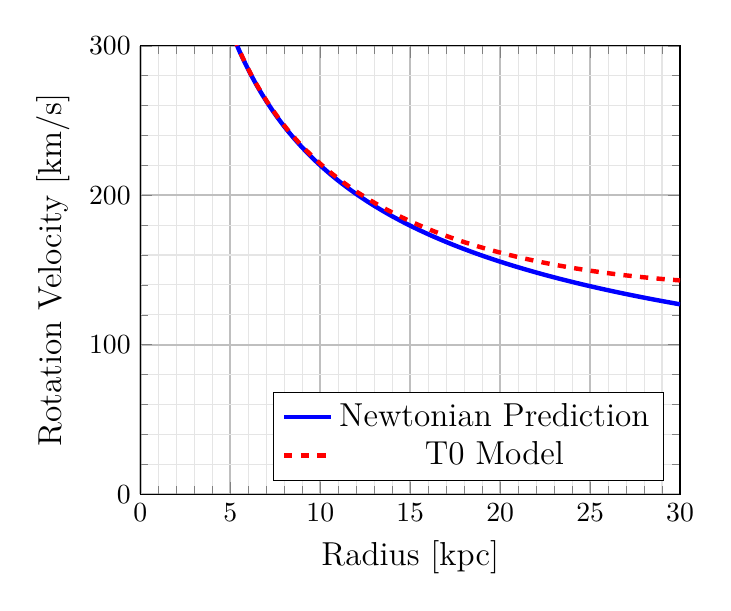
\begin{tikzpicture}
			\begin{axis}[
				xlabel={Radius [kpc]},
				ylabel={Rotation Velocity [km/s]},
				xlabel style={font=\large},
				ylabel style={font=\large},
				tick label style={font=\normalsize},
				xmin=0, xmax=30,
				ymin=0, ymax=300,
				legend pos=south east,
				legend style={font=\large},
				grid=both,
				minor tick num=4,
				major grid style={line width=0.8pt, gray!50},
				minor grid style={line width=0.4pt, gray!20}
				]
				\addplot[blue, ultra thick, domain=0.1:30, samples=100] {220*sqrt(10/x)};
				\addplot[red, dashed, ultra thick, domain=0.1:30, samples=100] {sqrt(220^2*10/x + 4.8*x^2)};
				\legend{Newtonian Prediction, T0 Model}
			\end{axis}
		\end{tikzpicture}
		\caption{Rotation curves with \(\kappa_{\text{SI}}\).}
	\end{figure}
	
	\begin{figure}[ht]
		\centering
		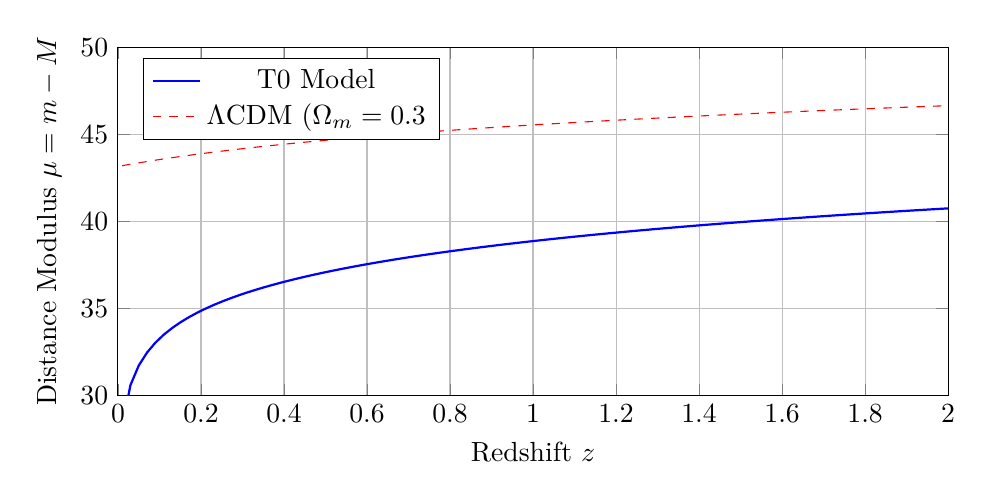
\begin{tikzpicture}
			\begin{axis}[
				xlabel={Redshift $z$},
				ylabel={Distance Modulus $\mu = m-M$},
				xmin=0,
				xmax=2,
				ymin=30,
				ymax=50,
				legend pos=north west,
				grid=both,
				width=\textwidth,
				height=6cm,
				samples=100
				]
				\addplot[blue, thick, domain=0.01:2] {5*log10(3e8/70e3*ln(1+x)*(1+x)*0.1) + 25}; % T0, steeper at high z
				\addplot[red, dashed, domain=0.01:2] {5*log10(3e8/70e3*(1+x)*(2-(1/(1+x)))*1) + 25}; % LCDM, flatter at high z
				\legend{T0 Model, $\Lambda$CDM ($\Omega_m=0.3$, $\Omega_{\Lambda}=0.7$)}
			\end{axis}
		\end{tikzpicture}
		\caption{Distance modulus vs. redshift
			comparing the T0 model prediction (solid blue)
			with the $\Lambda$CDM prediction (dashed red)
			for $H_0 = 70$ km/s/Mpc.
			The models show a distinctive pattern: initially far apart at low redshifts,
			they gradually converge at higher redshifts,
			providing a clear observational test.}
		\label{fig:distance_modulus}
	\end{figure}
	
	\section{Consequences of Setting \(\beta = 1\)}
	
	\subsection{Theoretical Elegance}
	
	\begin{itemize}
		\item Simplicity of the temperature-redshift relation
		\item Coherence of dimensionless parameters
		\item Clarity of relationships between fundamental quantities
	\end{itemize}
	
	\subsection{Conversion to SI Units}
	
	The conversion formula:
	\begin{equation}
		\betaT^{\text{SI}} = \betaT^{\text{nat}} \cdot \frac{\xi \cdot l_{P,\text{SI}}}{r_{0,\text{SI}}}
	\end{equation}
	
	This is analogous to \(c = 1\) in the theory of relativity, where we can switch between the theoretical formulation with \(c = 1\) and the experimental measurement with \(c = \SI{3e8}{\meter\per\second}\).
	
	\subsection{Reassessment of Measurements}
	
	The redshift discrepancy between predictions with \(\betaT^{\text{nat}} = 1\) and current "measured" values could indicate a standard model bias in the interpretation of cosmological data. It should be noted that:
	\begin{itemize}
		\item Cosmological measurements are typically calibrated within the framework of the \(\Lambda\)CDM model
		\item The "measured" values may contain implicit assumptions
		\item A complete reassessment within the framework of the T0 model with \(\betaT^{\text{nat}} = 1\) could lead to a consistent interpretation
	\end{itemize}
	
	The quantitative effects of this reassessment are analyzed in detail in \cite{pascher_alphabeta_2025}.
	
	\section{Integration into the Time-Mass Duality Theory}
	
	\subsection{Consistency with the Basic Principles}
	
	Setting \(\betaT^{\text{nat}} = 1\) is consistent with the basic principles of the time-mass duality theory:
	\begin{itemize}
		\item Time is absolute: The fundamental time scale is determined by the intrinsic time field \(\Tfield\)
		\item Mass varies: \(m = \frac{\hbar}{\Tfield c^2}\), whereby the variation is mediated by the Higgs field
		\item Emergent gravitation: Gravitation arises from the gradients of \(\Tfield\)
	\end{itemize}
	
	\subsection{Implications for Other Parameters}
	
	Setting \(\betaT^{\text{nat}} = 1\) affects other parameters of the T0 model, in particular:
	\begin{itemize}
		\item \(\kappa\): Direct dependence through the equation \(\kappa^{\text{nat}} = \frac{y v}{r_g^2}\)
		\item \(\alpha\): Connection through the characteristic length scales \(r_0\) and \(L_T\)
	\end{itemize}
	
	\section{Experimental Tests and Perspectives}
	
	\subsection{Direct Tests of Setting \(\beta = 1\)}
	
	\begin{itemize}
		\item \textbf{Precision measurements of the CMB spectrum:} A detailed analysis of deviations from the perfect blackbody spectrum could provide indications of the true form of the temperature-redshift relation.
		\item \textbf{Search for signatures of higher temperatures in the early cosmic history:} The investigation of isotope distributions from primordial nucleosynthesis could provide evidence for higher temperatures.
		\item \textbf{Direct temperature measurements at medium redshifts:} The deviation between the models increases with \(z\) and could already be measurable at medium redshifts.
	\end{itemize}
	
	\subsection{Indirect Tests and Cosmological Parameters}
	
	\begin{itemize}
		\item \textbf{Hubble tension:} A reinterpretation of the CMB data with \(\betaT^{\text{nat}} = 1\) could solve the Hubble tension problem.
		\item \textbf{Baryon Acoustic Oscillations (BAO):} \\The modified temperature-redshift relation would influence the interpretation of BAO measurements.
		\item \textbf{Galaxy formation:} Higher temperatures in the early universe would influence structure and galaxy formation.
	\end{itemize}
	
	For a detailed quantitative analysis of these tests, see \cite{pascher_alphabeta_2025}, where specific predictions and comparisons with the standard model are presented.
	
	\section{Conclusions}
	
	Setting \(\betaT^{\text{nat}} = 1\) in natural units of the T0 model represents a conceptually elegant and physically motivated simplification, analogous to setting \(c = 1\) in the theory of relativity or \(\hbar = 1\) in quantum mechanics. This simplification requires a specific interpretation of the characteristic length scale \(r_0\) as \(r_0 \approx 1.33 \times 10^{-4} \cdot l_P\), which corresponds to a specific ratio to the Planck length.
	
	The resulting discrepancy with current "measurements" can be understood as an indication that our interpretation of cosmological data may be too strongly influenced by the paradigmatic framework of the standard model. This opens the door for new perspectives and experimental tests that could distinguish between different cosmological models.
	
	For practical application and comparison with experimental data, all results can be easily translated back into SI units. The conceptual elegance of a theory with simple dimensionless parameters (\(\betaT^{\text{nat}} = 1\)) versus complex values (\(\betaT^{\text{SI}} \approx 0.008\)) supports a deeper investigation of this possibility, especially in the context of the time-mass duality theory, which already proposes fundamental reinterpretations of physical concepts.
	
	\begin{thebibliography}{99}
		\bibitem{pascher_messdifferenzen_2025} Pascher, J. (2025). \href{https://github.com/jpascher/T0-Time-Mass-Duality/tree/main/2/pdf/English/MessdifferenzenT0StandardEn.pdf}{Compensatory and Additive Effects: An Analysis of Measurement Differences Between the T0 Model and the \(\Lambda\)CDM Standard Model}. April 2, 2025.
		\bibitem{pascher_temp_2025} Pascher, J. (2025). \href{https://github.com/jpascher/T0-Time-Mass-Duality/tree/main/2/pdf/English/TempEinheitenCMBEn.pdf}{Adjustment of Temperature Units in Natural Units and CMB Measurements}. April 2, 2025.
		
		
		
		
		\bibitem{pascher_galaxies_2025} Pascher, J. (2025). \href{https://github.com/jpascher/T0-Time-Mass-Duality/tree/main/2/pdf/English/MassVarGalaxienEn.pdf}{Mass Variation in Galaxies: An Analysis in the T0 Model with Emergent Gravitation}. March 30, 2025.
		\bibitem{pascher_params_2025} Pascher, J. (2025). \href{https://github.com/jpascher/T0-Time-Mass-Duality/tree/main/2/pdf/English/ZeitMasseT0ParamsEn.pdf}{Time-Mass Duality Theory (T0 Model): Derivation of Parameters \(\kappa\), \(\alpha\) and \(\beta\)}. March 30, 2025.
		\bibitem{pascher_alpha_2025} Pascher, J. (2025). \href{https://github.com/jpascher/T0-Time-Mass-Duality/tree/main/2/pdf/English/NatEinheitenAlpha1En.pdf}{Energy as Fundamental Unit: Natural Units with \(\alpha = 1\) in the T0 Model}. March 26, 2025.
		\bibitem{pascher_alphabeta_2025} Pascher, J. (2025). \href{https://github.com/jpascher/T0-Time-Mass-Duality/tree/main/2/pdf/English/Alpha1Beta1KonsistenzEn.pdf}{Unified Unit System in the T0 Model: The Consistency of \(\alpha = 1\) and \(\beta = 1\)}. April 5, 2025.
		\bibitem{pascher_zeit_2025} Pascher, J. (2025). \href{https://github.com/jpascher/T0-Time-Mass-Duality/tree/main/2/pdf/English/ZeitEmergentQMEn.pdf}{Time as an Emergent Property in Quantum Mechanics: A Connection Between Relativity, Fine Structure Constant, and Quantum Dynamics}. March 23, 2025.
		\bibitem{pascher_higgs_2025} Pascher, J. (2025). \href{https://github.com/jpascher/T0-Time-Mass-Duality/tree/main/2/pdf/English/MathHiggsZeitMasseEn.pdf}{Mathematical Formulation of the Higgs Mechanism in Time-Mass Duality}. March 28, 2025.
		\bibitem{pascher_lagrange_2025} Pascher, J. (2025). \href{https://github.com/jpascher/T0-Time-Mass-Duality/tree/main/2/pdf/English/MathZeitMasseLagrange.pdf}{From Time Dilation to Mass Variation: Mathematical Core Formulations of Time-Mass Duality Theory}. March 29, 2025.
		
		\bibitem{pascher_emergente_gravitation_2025} Pascher, J. (2025). \href{https://github.com/jpascher/T0-Time-Mass-Duality/tree/main/2/pdf/English/EmergentGravT0En.pdf}{Emergent Gravitation in the T0 Model: A Comprehensive Derivation}. April 1, 2025.
		\bibitem{pascher_feldtheorie_2025} Pascher, J. (2025). \href{https://github.com/jpascher/T0-Time-Mass-Duality/tree/main/2/pdf/English/FeldtheorieQuantenEn.pdf}{Field Theory and Quantum Correlations: A New Perspective on Instantaneity}. March 28, 2025.
		\bibitem{pascher_planck_2025} Pascher, J. (2025). \href{https://github.com/jpascher/T0-Time-Mass-Duality/tree/main/2/pdf/English/JenseitsPlanckEn.pdf}{Real Consequences of Reformulating Time and Mass in Physics: Beyond the Planck Scale}. March 24, 2025.
		\bibitem{pascher_erweiterung_2025} Pascher, J. (2025). \href{https://github.com/jpascher/T0-Time-Mass-Duality/tree/main/2/pdf/English/NotwendigkeitQMErweiterungEn.pdf}{The Necessity of Extending Standard Quantum Mechanics and Quantum Field Theory}. March 27, 2025.
		\bibitem{pascher_energiedynamik_2025} Pascher, J. (2025). \href{https://github.com/jpascher/T0-Time-Mass-Duality/tree/main/2/pdf/English/MathEnergiedynamikEn.pdf}{Dark Energy in the T0 Model: A Mathematical Analysis of Energy Dynamics}. April 3, 2025.
		\bibitem{pascher_vereinheitlichung_2025} Pascher, J. (2025). \href{https://github.com/jpascher/T0-Time-Mass-Duality/tree/main/2/pdf/English/T0VereinheitlichungDEGalEn.pdf}{Unification of the T0 Model: Foundations, Dark Energy, and Galaxy Dynamics}. April 4, 2025.
		\bibitem{pascher_formalismen_2025} Pascher, J. (2025). \href{https://github.com/jpascher/T0-Time-Mass-Duality/tree/main/2/pdf/English/MathZeitMasseLagrangeEn.pdf}{From Time Dilation to Mass Variation: Mathematical Core Formulations of Time-Mass Duality Theory}. April 5, 2025.
		\bibitem{pascher_perspektive_2025} Pascher, J. (2025). \href{https://github.com/jpascher/T0-Time-Mass-Duality/tree/main/2/pdf/English/ZeitRaumPascher.pdf}{A New Perspective on Time and Space: Johann Pascher's Revolutionary Ideas}. March 25, 2025.
		\bibitem{pascher_dualismus_2025} Pascher, J. (2025). \href{https://github.com/jpascher/T0-Time-Mass-Duality/tree/main/2/pdf/English/KurzKomplementDualPhysikEn.pdf}{In Brief - Complementary Dualism in Physics: From Wave-Particle to Time-Mass Concept}. March 26, 2025.
		\bibitem{pascher_grundkraefte_2025} Pascher, J. (2025). \href{https://github.com/jpascher/T0-Time-Mass-Duality/tree/main/2/pdf/English/VierKraefteZeitMasse.pdf}{Simplified Description of the Fundamental Forces with Time-Mass Duality}. March 27, 2025.
		\bibitem{pascher_zeit_masse_2025} Pascher, J. (2025). \href{https://github.com/jpascher/T0-Time-Mass-Duality/tree/main/2/pdf/English/ZeitMasseNeuerBlickEn.pdf}{Time and Mass: A New Look at Old Formulas - and Liberation from Traditional Constraints}. March 22, 2025.
		\bibitem{Planck1899} Planck, M. (1899). On Irreversible Radiation Processes. \textit{Sitzungsberichte der Preußischen Akademie der Wissenschaften}, 5, 440-480.
		\bibitem{Feynman1985} Feynman, R. P. (1985). \textit{QED: The Strange Theory of Light and Matter}. Princeton University Press.
		\bibitem{Duff2002} Duff, M. J., Okun, L. B., \& Veneziano, G. (2002). \textit{Trialogue on the Number of Fundamental Constants}. \textit{Journal of High Energy Physics}, 2002(03), 023.
		\bibitem{Verlinde2011} Verlinde, E. (2011). \textit{On the Origin of Gravity and Newton's Laws}. \textit{Journal of High Energy Physics}, 2011(4), 29.
		\bibitem{Wilczek2008} Wilczek, F. (2008). \textit{The Lightness of Being: Mass, Ether, and the Unification of Forces}. Basic Books.
		\bibitem{DiracLargeNumbers} Dirac, P. A. M. (1937). The Cosmological Constants. \textit{Nature}, 139, 323.
		\bibitem{Eddington1946} Eddington, A. S. (1946). \textit{Fundamental Theory}. Cambridge University Press.
		\bibitem{WeinbergAsymSafety} Weinberg, S. (1979). Ultraviolet divergences in quantum theories of gravitation. In \textit{General Relativity: An Einstein Centenary Survey}, ed. S. W. Hawking and W. Israel, Cambridge University Press, pp. 790-831.
		\bibitem{tHooft1993} 't Hooft, G. (1993). Dimensional reduction in quantum gravity. In \textit{Salamfestschrift: A Collection of Talks}, World Scientific Series in 20th Century Physics, vol. 4, ed. A. Ali, J. Ellis, and S. Randjbar-Daemi, World Scientific, pp. 284-296.
		\bibitem{Planck2018Temp} Planck Collaboration, Aghanim, N., et al. (2020). \textit{Planck 2018 Results. V. CMB Power Spectra and Likelihoods}. \textit{Astronomy \& Astrophysics}, 641, A5. DOI: 10.1051/0004-6361/201833887.
		\bibitem{Fixsen2009} Fixsen, D. J. (2009). \textit{The Temperature of the Cosmic Microwave Background}. \textit{The Astrophysical Journal}, 707(2), 916-920. DOI: 10.1088/0004-637X/707/2/916.
		\bibitem{ACTTemp} Choi, S. K., et al. (2020). \textit{The Atacama Cosmology Telescope: A Measurement of the Cosmic Microwave Background Power Spectra at 98 and 150 GHz}. \textit{Journal of Cosmology and Astroparticle Physics}, 2020(12), 045. DOI: 10.1088/1475-7516/2020/12/045.
		\bibitem{SPTTemp} Reichardt, C. L., et al. (2021). \textit{The South Pole Telescope 3G Survey: Cosmic Microwave Background Temperature and Polarization Power Spectra}. \textit{The Astrophysical Journal}, 908(2), 199. DOI: 10.3847/1538-4357/abd407.
		\bibitem{Mather1994} Mather, J. C., et al. (1994). \textit{Measurement of the Cosmic Microwave Background Spectrum by the COBE FIRAS Instrument}. \textit{The Astrophysical Journal}, 420, 439-444. DOI: 10.1086/173574.
		\bibitem{SunyaevZeldovich} Birkinshaw, M. (1999). \textit{The Sunyaev-Zel'dovich Effect}. \textit{Physics Reports}, 310(2-3), 97-195. DOI: 10.1016/S0370-1573(98)00080-5.
		\bibitem{PlanckTech} Planck Collaboration, Tauber, J. A., et al. (2010). \textit{Planck Pre-launch Status: The Planck Mission}. \textit{Astronomy \& Astrophysics}, 520, A1. DOI: 10.1051/0004-6361/200912983.
		\bibitem{CMBTheoryTemp} Hu, W., \& Dodelson, S. (2002). \textit{Cosmic Microwave Background Anisotropies}. \textit{Annual Review of Astronomy and Astrophysics}, 40, 171-216. DOI: 10.1146/annurev.astro.40.060401.093926.
		\bibitem{Einstein1915} Einstein, A. (1915). The Field Equations of Gravitation. \textit{Sitzungsberichte der Preussischen Akademie der Wissenschaften zu Berlin}, 844-847.
		\bibitem{Higgs1964} Higgs, P. W. (1964). Broken Symmetries and the Masses of Gauge Bosons. \textit{Physical Review Letters}, 13(16), 508-509.
		\bibitem{Will2014} Will, C. M. (2014). The Confrontation between General Relativity and Experiment. \textit{Living Reviews in Relativity}, 17(1), 4.
	\end{thebibliography}
	
\end{document}
